Suppose that there are two species in competition with one another in an environment where the common food supply is limited.
For example, sea lions and penguins, red and gray squirrels, and ants and termites are all species which fall into this category.\\
There are two particular types of outcome that are often observed in the real world.
In the first case, there is coexistence, in which the two species live in harmony.
(In nature, this is the most likely outcome; otherwise, one of the species would be extinct.)
In the second case, there is mutual exclusion, in which one of the species becomes extinct. (For example, American gray squirrels imported into the UK are causing the extinction of the smaller native red squirrels.)
The Equations are given by
\begin{equation}{\label{eq:cs}}
	\begin{aligned}
		\dot{x}=x(\beta-\delta x-\gamma y)\\
		\dot{y}=y(b-dy-cx)
	\end{aligned}
\end{equation}
where $\beta,\delta,\gamma,a,b,c$ are all positive constants with $x(t)$ and $y(t)$ both positive representing the two species populations measured.\\
Physical Meaning:
\begin{itemize}
	\item The terms $\beta x-\delta x^2$ and $by-dy^2$ represent the usual logistic growth of one species.
	\item Both species suffer as a result of competition over a limited food supply, hence the terms $-\gamma xy$ and $-cxy$ in $\dot{x}$ and $\dot{y}$.
\end{itemize}
Fixed points of equation (\ref{eq:cs}) are
\begin{equation}
	O=(0,0),\quad P=\left(0,\frac{b}{d}\right),\quad Q=\left(\frac{\beta}{\delta},0\right),\quad and\quad R=\left(\frac{\gamma b-\beta d}{\gamma c-\delta d},\frac{\beta c-\delta b}{\gamma c-\delta d}\right)
\end{equation}
Suppose that $C_1=\gamma c-\delta d$, $C_2=\gamma b-\beta d$,and $C_3=\gamma c-\delta d$.
For the fixed point to lie in the first quadrant, one of the following conditions must hold:
\begin{enumerate}[label=(\roman*)]
	\item $C_1$,$C_2$, and $C_3$ are all negative.
	\item $C_1$,$C_2$, and $C_3$ are all positive.
\end{enumerate}
Linearize by finding the Jacobian matrix.
\begin{equation}
	J=
	\begin{pmatrix}
		\beta-2\delta x-\gamma y&-\gamma x\\
		-cy&b-2dy-cx
	\end{pmatrix}
\end{equation}
$J$ at each fixed point is
\begin{equation*}
	J_O=
	\begin{pmatrix}
		\beta&0\\0&b
	\end{pmatrix}\quad
	J_P=
	\begin{pmatrix}
		\beta-\gamma b/d&0\\
		-bc/d&-b
	\end{pmatrix}\quad
	J_Q=
	\begin{pmatrix}
		-\beta&-\gamma \beta/\delta\\
		0&b-\beta c/\delta
	\end{pmatrix}\quad
	J_R=\frac{1}{C_1}
	\begin{pmatrix}
		\delta C_2&\gamma C_2\\
		cC_3&dC_3
	\end{pmatrix}
\end{equation*}
Let's Consider case (i) first.
The fixed points are all simple, and it is not difficult
to show that $O$ is an unstable node, $P$ and $Q$ are cols, and for certain parameter values $R$ is a stable fixed point.
A phase portrait is plotted in Figure (\ref{fig:cs}a), where eight of an infinite number of solution curves are plotted.
For the parameter values chosen here, the two species coexist and the populations stabilize to constant values after long time periods.
The arrows in the Figure (\ref{fig:cs}a) show the vector field plot and define the direction of the trajectories for system (\ref{fig:cs}a).
There is a stable node lying wholly in the first quadrant at $R$, and the nonzero populations $x(t)$ and $y(t)$ tend to this critical point with increasing time no matter what the initial populations are.\\
\begin{figure}[H]
	\centering
	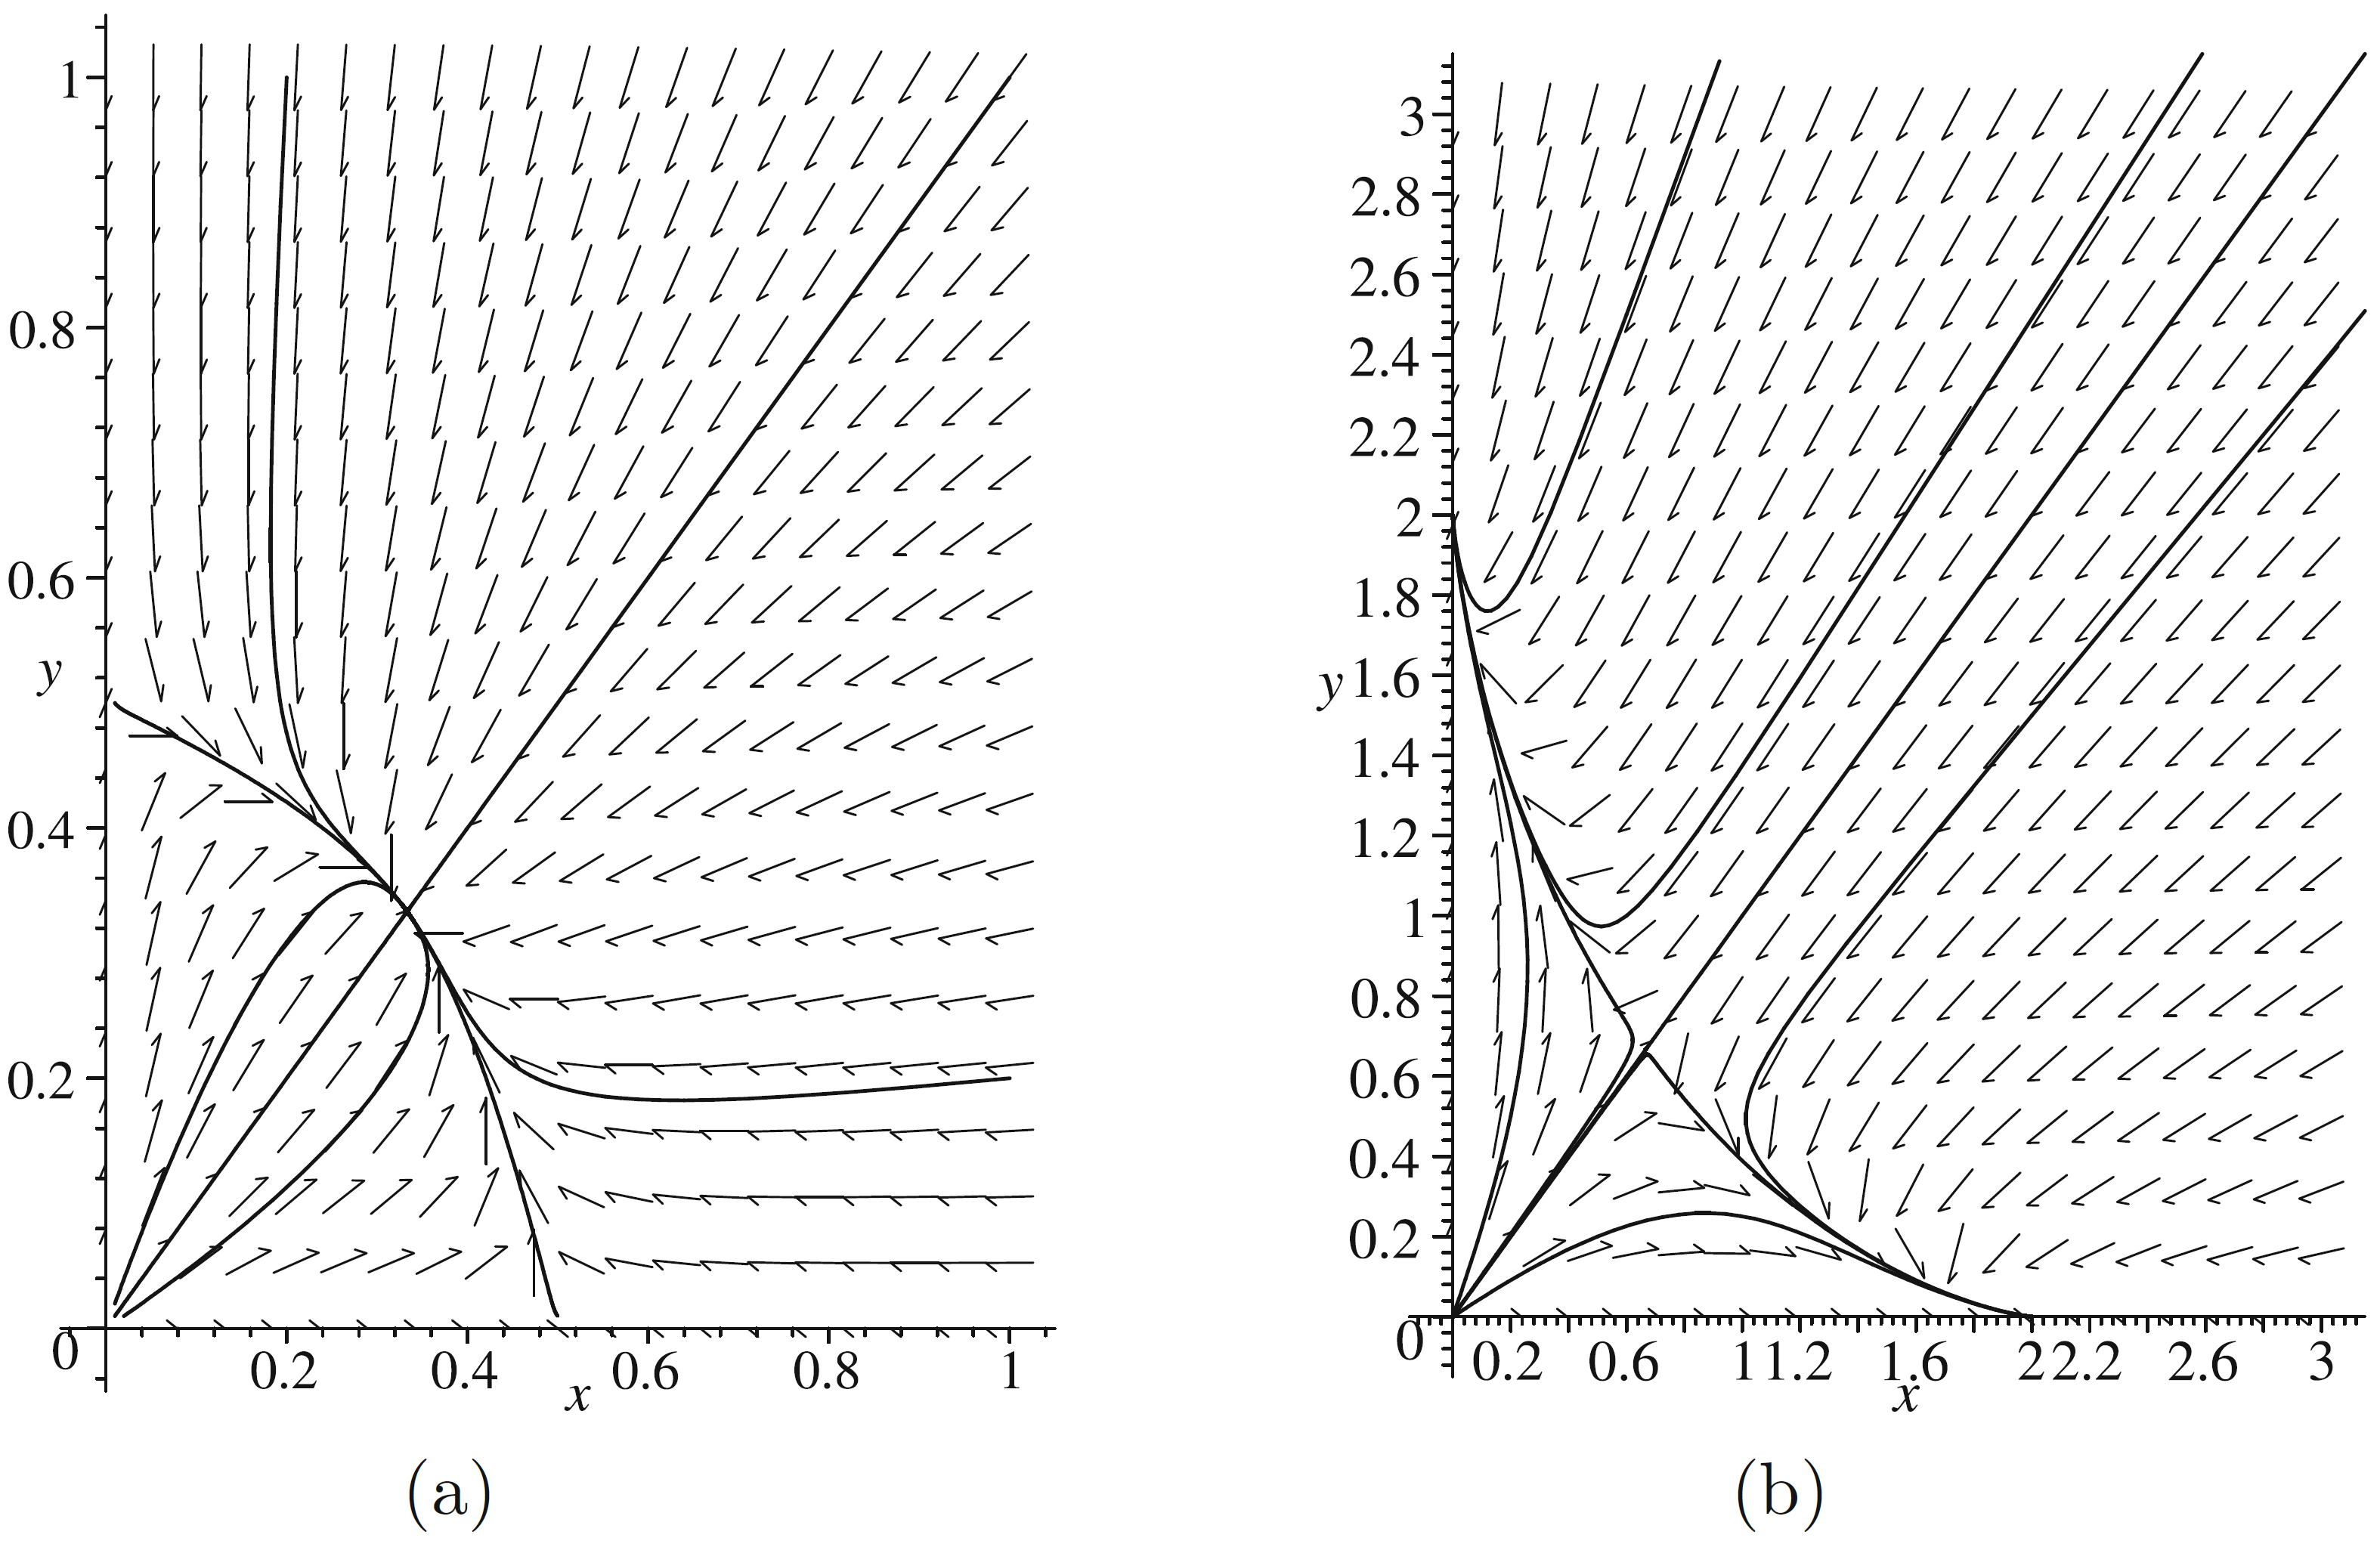
\includegraphics[width=0.6\linewidth]{cs.png}
	\caption{(a) A possible phase portrait showing coexistence.\\(b) A possible phase portrait depicting mutual exclusion.}
	\label{fig:cs}
\end{figure}
Now consider case (ii).
The fixed points are all simple, and it is not difficult to show that $O$ is an unstable node, $P$ and $Q$ are stable or improper nodes, and $R$ is a col.
A phase portrait is shown in Figure (\ref{fig:cs}b), where nine of an infinite number of solution curves are plotted.
In this case, one of the species becomes extinct.
In Figure (\ref{fig:cs}b), the critical point lying wholly in the first quadrant is a
saddle point or col, which is unstable.
The long-term behavior of the system is divided along the diagonal in the first quadrant.
Trajectories starting to the right of the diagonal will tend to the critical point at $Q =(2, 0)$, which implies that species $y$ becomes extinct
Trajectories starting to the left of the diagonal will tend to the critical point at $P =(0, 2)$, which means that species $x$ will become extinct.
Numerically, the trajectories lying on the stable manifold of the saddle point in the first quadrant will tend toward the critical point at $R$.
However, in the real world, populations cannot remain exactly on the stable manifold, and trajectories will be diverted from this critical point leading to extinction of one of the species.